\chapter{Literature Review}

This chapter reviews the currently available implementations of various
components in the processing pipeline. This chapter would be divided into
two sections, each dealing with a process --- the first section would
describe transcription, and the second section captioning.

Most of the implementations chosen are free, open-source and cross-platform.

\section{Transcription}

Figure~\ref{trans} provided the transcription pipeline of three components
--- a resampler, a diarizer and a transcription engine. We would go into
each component in detail.

Furthermore, to enable transcription of multi-channel recording, the concept
of voice-activity detection (VAD) would also be discussed.

\subsection{Resampling}

In the context of this project, resampling is concerned with converting an
audio stream from different specifications to a standard one, before passing to
other processing steps. Some common attributes of an audio stream are:

\begin{longtabu}{X[1.5,l]X[4,l]X[2.5,l]}
    \textbf{Attribute} & \textbf{Description} & \textbf{Examples} \\
    \midrule
    \endhead{}
    Sample rate &
    (defined for PCM audio)\newline Number of audio samples per
    second~\cite{weik1995communications} &
    CD audio: 44100 Hz~\cite{sample-rate} \\
    Bit depth &
    (defined for PCM audio)\newline Number of bits to represent
    a sample~\cite{thompson2005understanding} &
    CD audio: 16 bits~\cite{iec60908} \\
    Number of channels &
    Number of independent audio channels (to create a
    perception of depth) &
    Mono (1-channel)/\newline
    Stereo (2-channel)~\cite{mono-stereo} \\
    Audio coding format &
    The specific encoder/ decoder used to create the audio stream;
    usually associated with a certain file extension &
    MPEG-2 Audio Layer III (\texttt{.mp3})~\cite{mp3}\newline
    WAVE (\texttt{.wav})~\cite{wav} \\
    \caption{Common audio stream attributes}
\end{longtabu}

Respectively, in order to resample audio streams, the following tasks
are performed on the original audio stream\footnote{The canonical
definition of resampling is only concerned with the first task
(sample rate conversion).}:

\begin{itemize}
    \item Sample rate conversion --- changing the sample rate of the audio
    (for instance, from 44100Hz to 16000Hz)
    \item Sample format conversion --- changing the type of the sample
    (for instance, from 16-bit to 8-bit samples)
    \item Channel rematrixing --- changing the number of channels
    (for instance, from stereo to mono audio)
    \item Transcoding --- changing the audio coding format (for instance,
    from WAVE to MPEG Layer-3)
\end{itemize}

There are two software packages to perform all the above tasks:

\subsubsection{Sound eXchange --- SoX (\texttt{sox})}

SoX is a cross-platform command-line utility that supports conversion
between a wide range of audio formats. Additionally, the utility could
apply effects, and play and record audio files~\cite{sox-docs}.
SoX is written in C\@; the associated library is \texttt{libsox}. Its
resampling library is released separately as
\texttt{libsoxr}~\cite{sox}.

\begin{figure}[h]
\begin{center}
    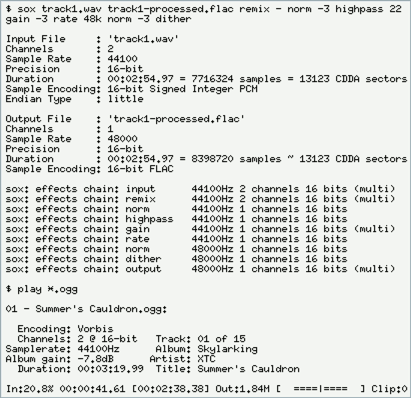
\includegraphics[width=0.6\textwidth]{sox}
    \caption{An example SoX session~\cite{sox}}
\end{center}
\end{figure}

The latest version of SoX, 14.4.2 was released in February 2015. The
current status of development work is uncertain; many issues and pull
requests are outstanding~\cite{sox-cl}.

\subsubsection{FFmpeg (\texttt{ffmpeg})}

FFmpeg is another C cross-platform utility to record, convert and stream
audio and video~\cite{ffmpeg}. FFmpeg provides a resampler which can
perform audio resampling, audio channel layout rematrixing, and convert
audio format and packing layout; it interfaces with its own resampling
library (\texttt{libswresample}) as well as SoX's resampling
library~\cite{ffmpeg-res,ffmpeg-libres}.

The library is actively developed; its latest stable version is 3.4
and it was released in October 2017~\cite{ffmpeg-dl}.

\subsubsection{Evaluation}

The two packages offer very similar functionalities; they are also
highly performant. However, FFmpeg has two clear advantages: it is
actively maintained and updated, and it operates on both audio and
video files (compare to audio only for SoX). FFmpeg also supports
more audio formats out-of-the-box.

Overall, FFmpeg would be a more suitable package for the project.

\subsection{Diarization}

With respect to an audio stream of multiple speakers, diarization is
the process of determining which speaker is speaking at when~\cite{diar}. 
Diarization is a combination of two tasks --- speaker segmentation,
which is the process of finding speaker change points in an audio stream,
to split the stream into smaller segments; and speaker clustering,
which is the process of grouping said segments based on speaker
characteristics, ideally resulting in one cluster per actual
speaker~\cite{diar-cls}.

One of the most frequently cited diarization toolkit is LIUM Speaker
Diarization.

\subsubsection{LIUM Speaker Diarization}

LIUM Speaker Diarization is an open-source diarization toolkit developed
at Laboratoire d'Informatique de l'Université du Maine~\cite{lium}.



It produces a segmentation file 
(\texttt{.seg})~\cite{lium-seg} which details the start time, end time and
\texttt{speaker\_id} of all identified segments. The source package is in Java;
however there is a convenient command-line interface~\cite{lium} which allows
for a Python wrapper (using the standard Python library module
\texttt{subprocess}).

\subsection{Transcription Engine}

The main purpose of the transcription engine is to transcribe speech
segments to text. There are a number of transcription engines available.

\subsubsection{Google Cloud Speech API}

Cloud Speech API~\cite{gcs} is developed by Google, providing the same speech
recognition capabilities powering Google's native applications (such as Voice
Search) to developers. A Python client library (\texttt{google-cloud-speech})
~\cite{gh-gcs} is available which would form the basis of the implemented module.
However to perform speech recognition, one needs to provide a Google API service
account key~\cite{gcs-api-key} and this key is used for usage tracking; the free
tier only allows \$300 of credits to be used in 12 months~\cite{gcs-free}
\footnote{Usage is charged in terms of 15-second blocks; each block is \$0.0025.}.
As such, care must be taken not to exceed the limit; complete checks are heavily
enforced to reduce the number of unnecessary API operations.

\subsection{Voice-activity Detection (VAD)}

In a multi-channel recording scenario.

\section{Captioning}